\documentclass[../main.tex]{subfiles}
The main hurdle to overcome in answering causal questions about the unsheltered homeless is that there is little data on their whereabouts. The Ending Community Homelessness Coalition of Austin (ECHO) conducts a yearly point-in-time (PIT) count of all the unsheltered people living in the city \cite{pit2020}. The irregularity of the sample makes it difficult to conduct meaningful inference, and the survey is subject to methodological issues (including, for instance, that the survey is conducted by volunteers and reliability is hence dependent on volunteer turnout).

Instead, I will try to conduct inference based on the anti-homeless citation data that I have. This means I will have to develop some stylized facts that describe the relationship between the issuance of citations and the location decisions of unsheltered people. An ideal model would allow for the number of citations issued in area \(i\) in time \(t\), \(cit_{it}\), to depend on the number of unsheltered people \(n_{it}\) and a policy variable \(p_{it}\):
\begin{equation*}
    cit_{it} = f(n_{it}, p_{it}, \varepsilon_{it}; \theta)
\end{equation*}
This captures the interplay between the policing policy that the City Council and Police Department set and the naturally tendency for certain parts of the city to be more attractive to unsheltered people. We would naturally expect
\begin{equation*}
    \frac{\partial cit_{it}}{\partial n_{it}}, \frac{\partial cit_{it}}{\partial p_{it}} > 0
\end{equation*}
as long as increasing \(p_{it}\) denotes a stricter policing policy. As reduced-form evidence, consider Figure~\ref{fig:citations_by_tract}. This shows the number of citations written monthly, by census tract. The PIT count notes that nearly 40\% of the entire unsheltered population resides within the Downtown area of Austin. This corresponds to the census tract 001100. Figure~\ref{fig:citations_by_tract} highlights this census tract, and it is at least anecdotally obvious that the number of citations is higher in this area of Austin where the unsheltered population tends to concentrate. Likewise, Figure~\ref{fig:citations_over_time} provides some anecdotal evidence that as the City Council relaxed their stance on the anti-homeless ordinances, the number of citations fell.

\begin{figure}[h]
    \begin{center}
        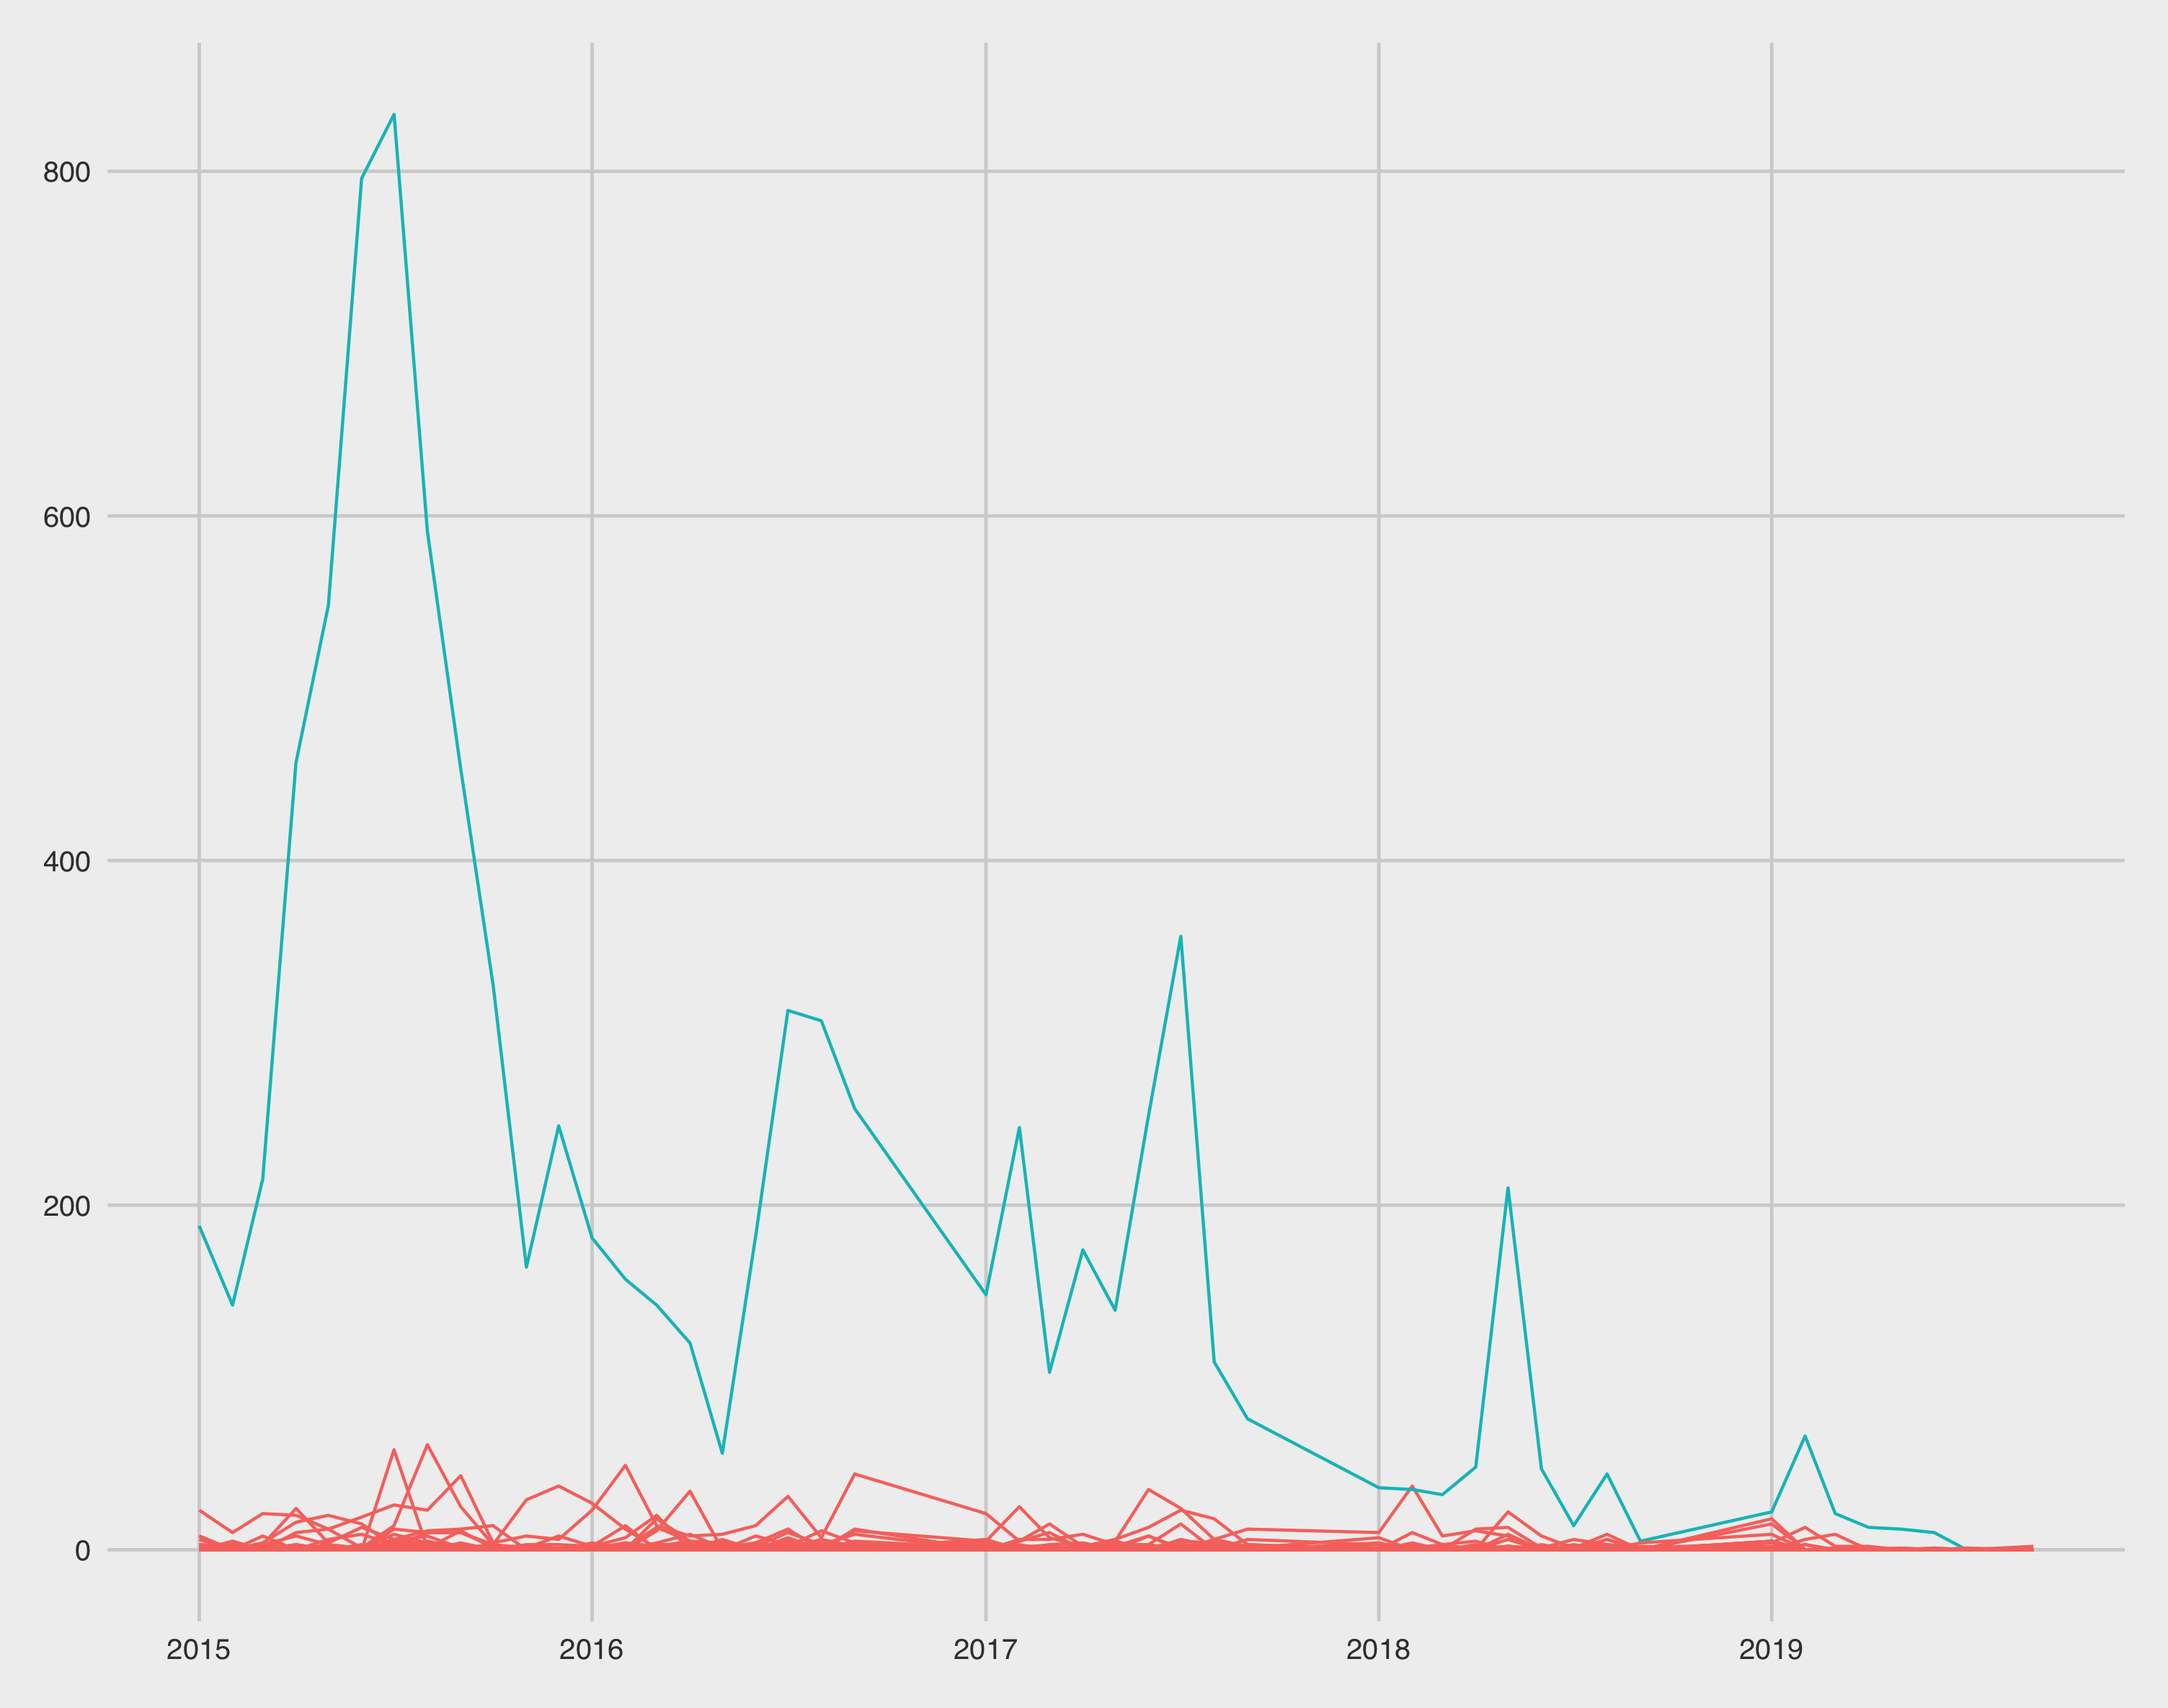
\includegraphics[width=.75\textwidth]{../../figures/monthly_citations.png}
        \caption{Monthly Ordinance Citations by Census Tract. Downtown (Census~Tract 001100) Highlighted}
        \label{fig:citations_by_tract}
    \end{center}
\end{figure}

More difficult to establish is the true deterrent effect that issuing citations has on unsheltered people. We may like to specify some intertemporal model of deterrence:
\begin{equation*}
    n_{it} = g(n_{i,t-1}, cit_{i, t-1}, \xi_{it}; \theta)
\end{equation*}

where there is state dependence, and citations written in a previous period will tend to deter people from residing in the same area in the next period:
\begin{equation*}
    \frac{\partial n_{it}}{\partial n_{i,t-1}} > 0, \frac{\partial n_{it}}{\partial cit_{i,t-1}} < 0
\end{equation*}

In practice, anecdotal evidence from the City Auditor's report may cast doubt on the strength of this deterrent effect. They report a high number of serial ordinance offenders who are repeatedly cited and refuse case management services. Some 65 individuals accounted for around 10\% of the 18,000 citations the auditor reviewed between 2014 and 2016, and the most egregious offender was cited more than 120 times in one year alone~\cite{ordinance_audit}.

I will generally assume then that a citation has a transitory deterrent impact. The PIT always finds that the same parts of Austin have the highest unsheltered counts, namely areas around downtown (see Figure~\ref{fig:pit_maps}). If enforcement policy had any permanent effect then this would not be the case. Rather, it seems that this is a strongly local effect, with the camping ban doing little to force relocation of people experiencing homelessness. Indeed, accounts from unsheltered people depict a life lived just out of sight in the numerous creeks and wild areas that permeate urban Austin~\cite{observer_article}\cite{eighner}. The geographic dispersion changes little.

\begin{figure}[h]
    \begin{center}
        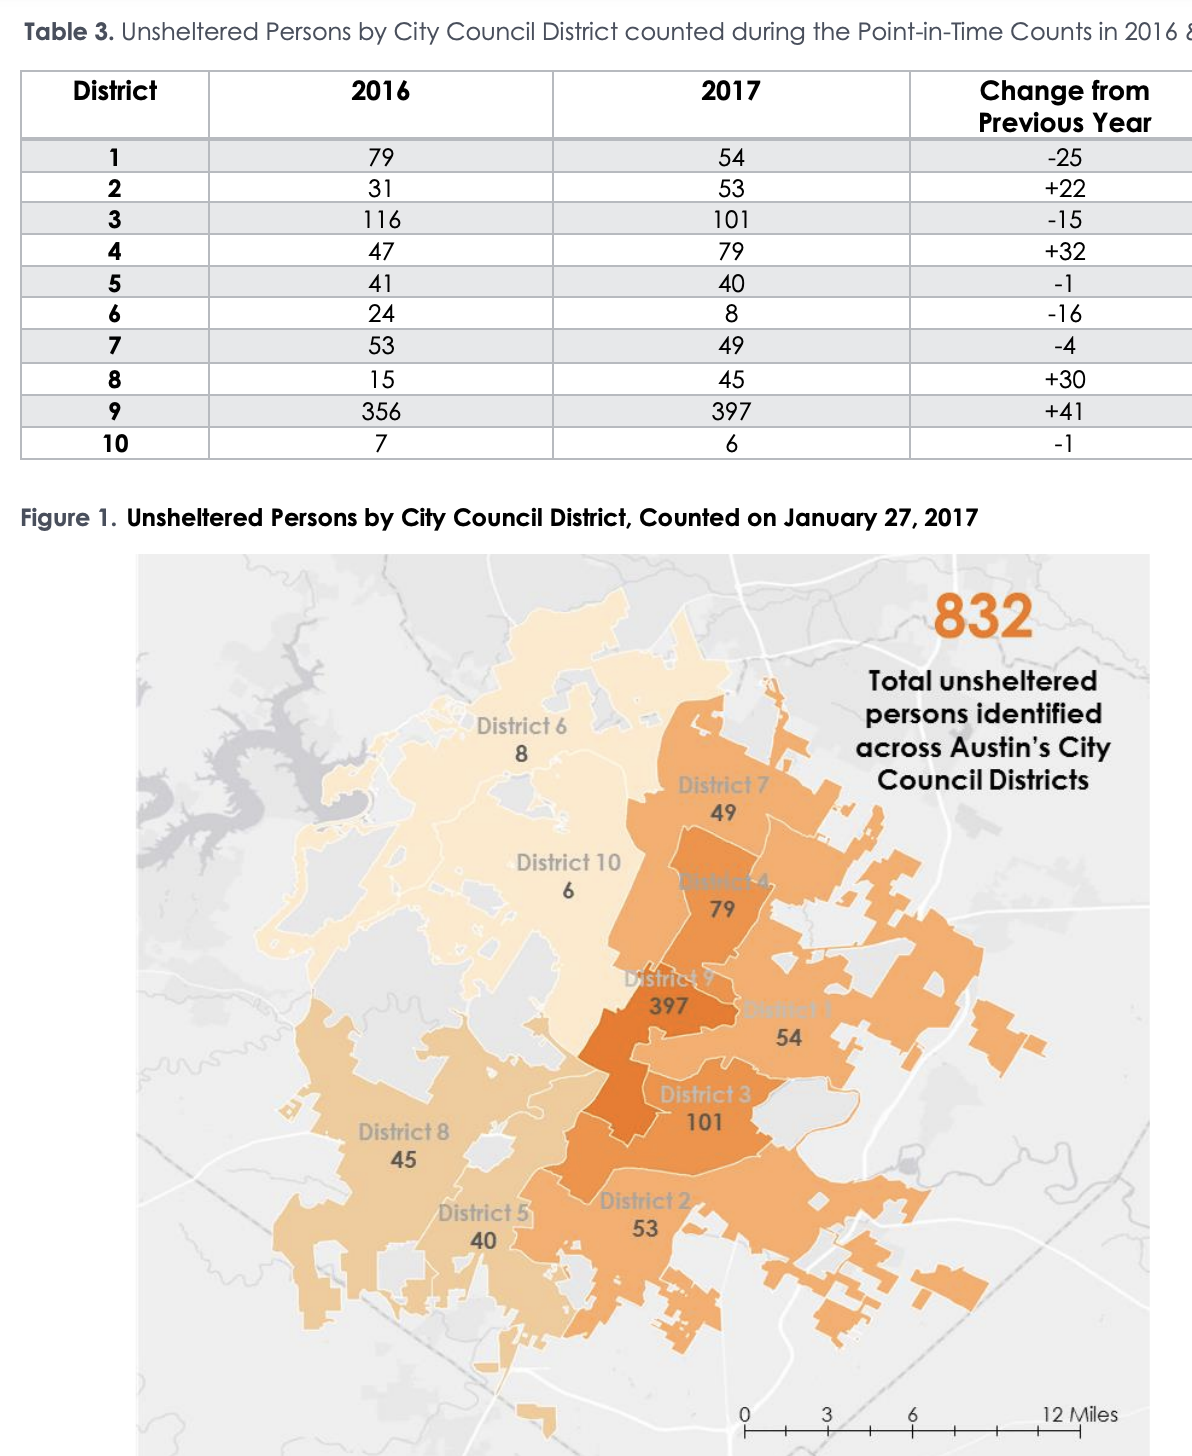
\includegraphics[width=.75\textwidth]{../../figures/pit_map.png}
        \caption{Select Figure from PIT Count 2017~\cite{pit2017}. City Council District 9, which represents Downtown Austin, accounts for majority of unsheltered count even amidst policy change.}
        \label{fig:pit_maps}
    \end{center}
\end{figure}

It is reasonable to question, then, what treatment effect we hope to isolate by comparing high-citation to low-citation areas of the city. If it is not a physical displacement, does it change unsheltered people's behavior? When trying to isolate the effect of the camping ban on crime, it is important to keep in mind this ambiguous treatment effect. In a sense, the causal mechanism is for proponents of the camping ban to define.

Ambiguity aside, we turn to a basic model of crime. Lacking time and data, I do not try to build on the rich literature on determinants of crime. Instead, I note that the demographic determinants that are often pointed to as integral are relatively immutable. So once again, I think of this as a primarily localized phenomenon. Figure~\ref{fig:crime_by_tract} shows monthly crime reports by census tract, with the downtown census tract 001100 again highlighted. In a reduced-form comparison of crime with and without the camping ban, I will assume that the within-tract variation in crimes committed captures the variation due to the (ambiguous) treatment induced by the City Council's camping ban repeal. Under this assumption, a fixed-effect model can yield a causal interpretation.

\begin{figure}[h]
    \begin{center}
        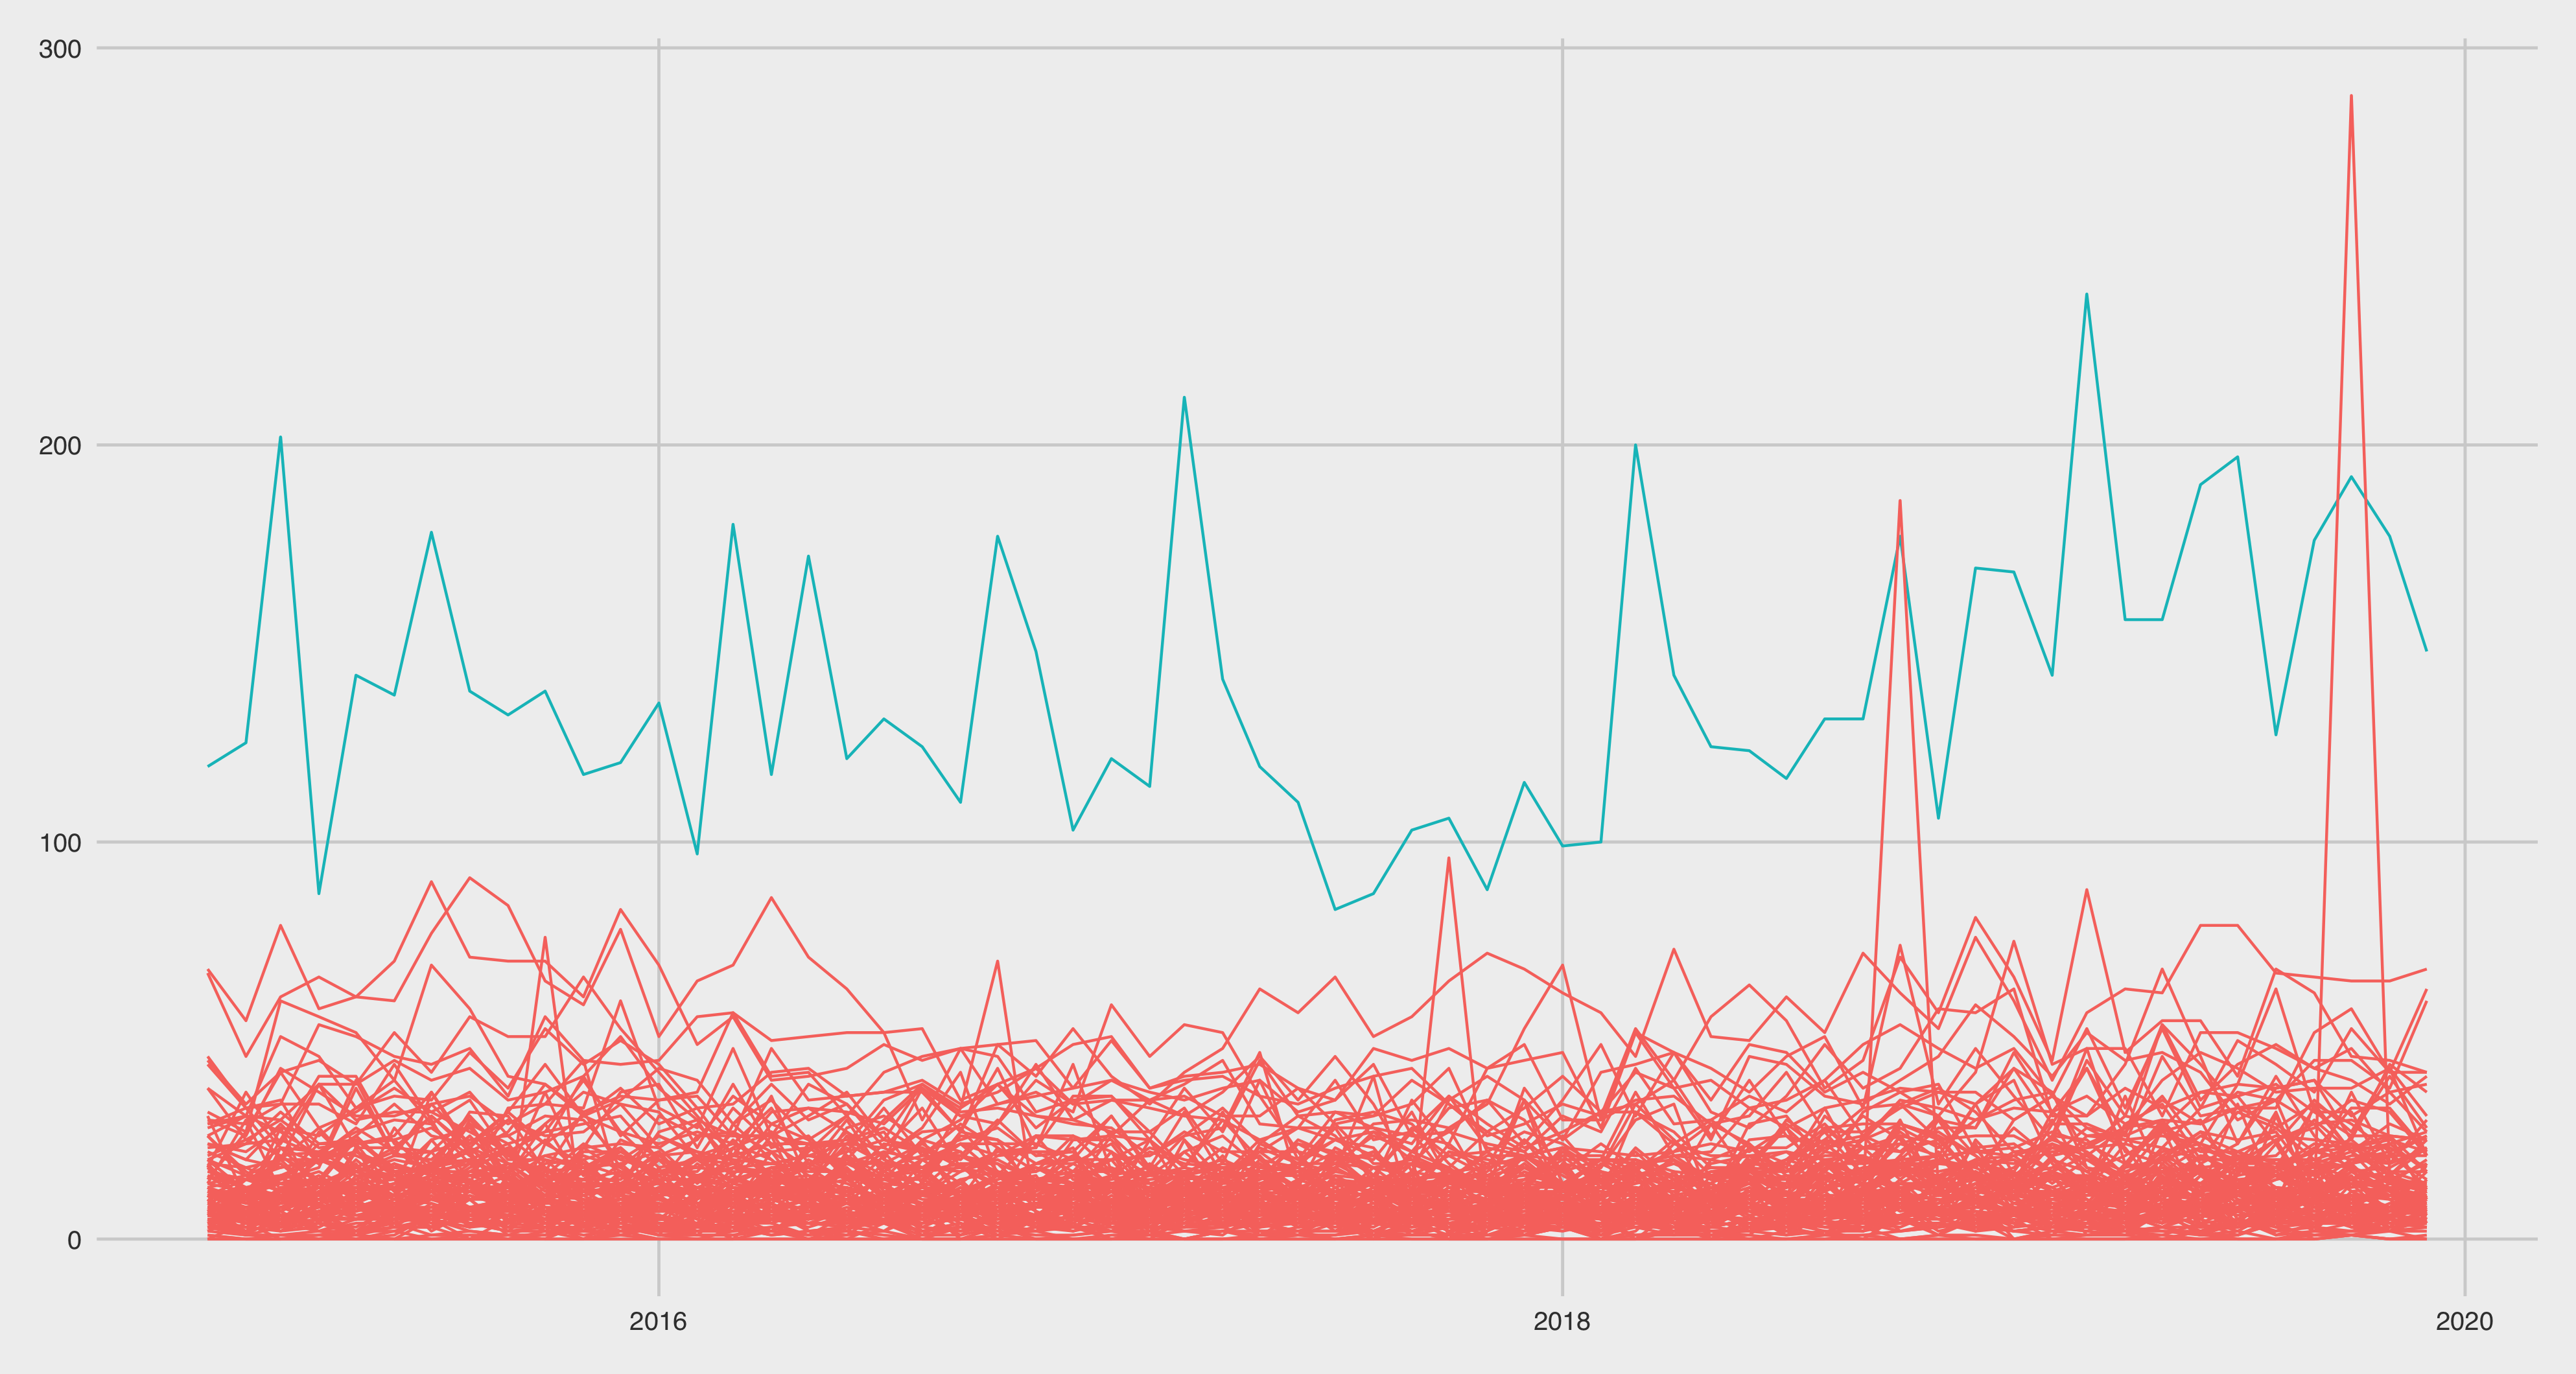
\includegraphics[width=.75\textwidth]{../../figures/crime_by_tract.png}
        \caption{Monthly Reports of Robbery and Theft, by census tract. Downtown Austin (001100) highlighted for distinction.}
        \label{fig:crime_by_tract}
    \end{center}
\end{figure}